%\VignetteIndexEntry{NCTools HowTo}
%\VignetteKeyword{platform}
%\VignettePackage{NCTools}
\documentclass[12pt]{article}
\usepackage{hyperref}
\usepackage{graphicx}
\textwidth=6.2in
\textheight=8.5in
%\parskip=.3cm
\oddsidemargin=.1in
\evensidemargin=.1in
\headheight=-.3in

\newcommand{\Robject}[1]{{\texttt{#1}}}
\newcommand{\Rfunction}[1]{{\texttt{#1}}}
\newcommand{\Rpackage}[1]{{\textit{#1}}}

\usepackage{/home/john/R-2.7.0/share/texmf/Sweave}
\begin{document}
\author{Jianhua Zhang}

\title{How to use CNTools}

\maketitle

\section*{Overview}

Studies have shown that genomic alterations measured as DNA copy number variations invariably occur across chromosomal regions that span over several genes, chromosome arms, or even whole chromosomes (reference). A common approach to analyzing DNA copy number data generated by microarrays, such as arrayCGH or SNP array, is to use the well established Circular Binary Segmentation (CBS) algorithm of the \Rpackage{DNAcopy} package to identify altered chromosome segments within each sample then find aberration accordant across samples. As samples usually differ in the number of altered regions and even for the same region where multiple samples show alterations the margins of the altered region rarely align across samples, the output of CBC can not be arranged as a matrix on which most computational algorithms operate. As the result, useful high level analysis such clustering or prediction can not be applied directly to segmented DNA copy number data.

The \Rpackage{CNTools} package provides the functionalities for converting the segmented DNA copy number data into a matrix format to facilitate further computational analyses. In this vignette, we show an example of clustering analysis using a public data set.  

\section*{Algothrims}

In the CNTools package, we implemented three algorithms of deriving a data set of matrix format that is referred to as reduced segment (RS) from now on for simplicity. First, by aligning chromosome segments across samples and then assigning segment means to overlapping chromosomal fragments (Figure 1) a reduced segment matrix (with the fragments as rows and samples as columns) can be obtained. This approach is straightforward but the drawback is the number of chromosomal fragments (or number of rows of the matrix) varies depending on the samples used for the calculation. Alternatively, by assigning segment means to genes within the segments for each sample a reduced segment matrix (with genes as rows and samples as columns) can be obtained. In this case the number of rows of the matrix does not vary with the samples of concern. Finally, by aligning chromosomal segments across each possible pair of samples a pair-wise reduced segment matrix can be obtained. The output is a list of reduced segment matrix derived from all the possible sample pairs. The data structure is only suitable for unsupervised classifications but not other computations such as supervised classifications.   

\begin{figure}[!htp]
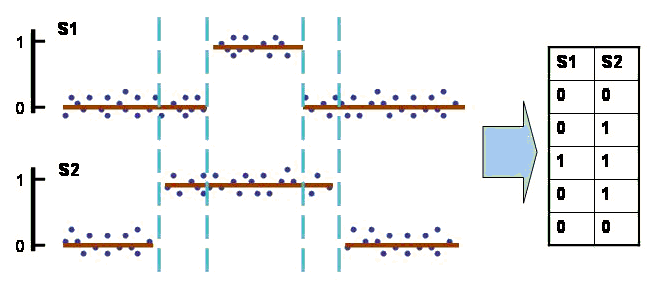
\includegraphics{fig01}
\begin{center}
\caption{Diagram showing how a reduced segment matrix is derived from segment data for two samples denoted as S1 and S2. Plue dots are probe log 2 ratios and red horizontal lines are the mean values for each identified segment. Vertical dashed lines indicate the edges of overlapping chromosome regions from which the matrix on the right}\label{fig:fig01}
\end{center}
\end{figure}

\section*{An example}

Here we use a public data set that is available from the TCGA data portal (\url{http://tcga-data.nci.nih.gov/tcga/homepage.htm}) to demonstrate the usage of the package. The data set contains 277 GBM tumor samples profiled using Agilent 244K density CGH array by the Harvard center. Normalized data were standardized by subtracting the median probe value of a sample from each probe log2 ratio of that sample before subjecting the data to the commonly used CBS algorithm available from the DNAcopy package of the Bioconductor (\url{http://www.bioconductor.org})project. The segment list was extracted from the CBS output and used as the source data for this package to obtain a reduced segment matrix. The extracted segment list is made available as part of the CNTools package and can be obtained by first loading the package and data set into an R session using the following R code:


The segment list is then used to instantiate a CNSeg object that is associated with methods to process the segment list data. The main method is getRS with the following parameters: 

\begin{itemize}
\item object: a CNSeg object containing the segment list of concern
\item by: a character string that can be either "region", "gene", or "pair" indicating which of the three algorithms to use to convert the data
\item input: a boolean of TRUE or FALSE to indicate whether missing values will be inputed
\item XY: a boolean of TRUE or FALSE to indicate whether data on the X and Y chromosomes will be included.
\end{itemize}

In this example, we elected to generate a reduced segment matrix of overlapping chromosomal regions without inputting missing values and drop data on the X and Y chromosomes (there are samples from both male and female patients in the data set). As the sample data contains more than 200 samples, in the example here, we use 20 of them due to speed consideration.

\begin{Schunk}
\begin{Sinput}
> cnseg <- CNSeg(sampleData[which(is.element(sampleData[, "ID"], 
+     sample(unique(sampleData[, "ID"]), 20))), ])
> rdseg <- getRS(cnseg, by = "region", input = FALSE, XY = FALSE)
\end{Sinput}
\begin{Soutput}
Processing samples ... Done
\end{Soutput}
\end{Schunk}

The rdseg obtained contains the reduced segment matrix and can be extracted by using the rs method if the uses prefer to pursue further computational analyses using their own code.

\begin{Schunk}
\begin{Sinput}
> reducedseg <- rs(rdseg)
\end{Sinput}
\end{Schunk}


However, the CNTools package provides functions to further process the data for further analyses. For classifications or differential tests, we wish to filter out features that do not vary much across samples. This can be done by calling the genefilter function of the genefilter package (assuming the filters are applicable to a matrix. Please read the documents of genefilter for detail). In the following code we show how to use a filter that is available from this package to retain the top 20% of the chromosome regions with the highest mean absolute deviation (MAD).

\begin{Schunk}
\begin{Sinput}
> filteredrs <- madFilter(rdseg, 0.8)
\end{Sinput}
\end{Schunk}

Now we call the dist function to calculate the similarities between samples using the Euclidian distance and then do a hierarchical clustering analysis using complete linkage for cluster agglomeration.



\begin{figure}[!htp]
\begin{center}
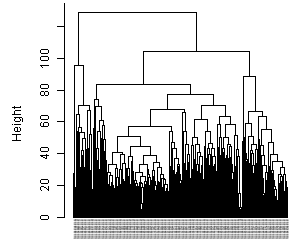
\includegraphics{fig02}
\caption{Dandrogram showing the clusters of all the samples containd in the sample data set}\label{fig:fig02}
\end{center}
\end{figure}

\end{document}

















